
\documentclass[letterpaper,10pt]{article}
\usepackage{amsmath}
\usepackage{amsfonts}
\usepackage{amssymb}
\usepackage{graphicx}
\usepackage[per-mode=symbol]{siunitx}
\usepackage[left=1in,right=1in,top=1in,bottom=1in]{geometry}
\usepackage{fancyhdr}
\usepackage{enumitem}
\usepackage[ampersand]{easylist}
\ListProperties(Numbers1=a,Numbers2=l,Progressive*=0.5cm,Hang=true,Space=0.2cm,Space*=0.2cm)

\setlength{\headheight}{0.5in}
\pagestyle{fancyplain}
\fancyhead[L]{Left Header}
\fancyhead[C]{Center Header}
\fancyhead[R]{Right Header}
\fancyfoot[L]{Left Footer}
\fancyfoot[C]{Center Footer}
\fancyfoot[R]{Right Footer}
\renewcommand{\headrulewidth}{0pt}

\setlength{\parindent}{0cm}

\title{the Title}
\author{}
\date{}

\begin{document}
\maketitle

\begin{minipage}{\linewidth}
  \begin{easylist}
  &  \label{prob_1} Does light travel faster or slower (compared to vacuum) in materials with a high refractive index? 
  \end{easylist}
\end{minipage}

Paragraphs can be used to put some text between questions

\begin{minipage}{\linewidth}
  \begin{easylist}
  &  \label{prob_2} Consider a ray of light that enters a piece of glass from air. 
    &&  \label{prob_2_1} If the ray is incident on the glass perpendicular to the surface, by what angle will it be bent? 
    &&  \label{prob_2_2} If the ray is incident on the glass at an angle of \SI{45}{\degree} to the surface, by what angle will it be bent? 
  \end{easylist}
\end{minipage}

but they cannot go between parts.

\begin{figure}
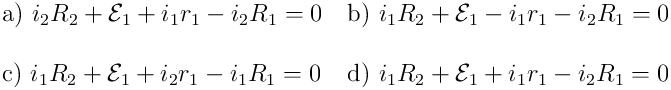
\includegraphics[]{picture.png}
\caption{ \label{fig:pic1} This is an example figure.}
\end{figure}
\begin{minipage}{\linewidth}
  \begin{easylist}
  &  \label{prob_3} What is the speed of light in water? 
  \end{easylist}
\end{minipage}
\begin{minipage}{\linewidth}
  \begin{easylist}
  &  \label{prob_5} Will the speed of light be faster in: 
    &&  \label{prob_5_1} glass or water? 
  \end{easylist}
\end{minipage}
\begin{figure}
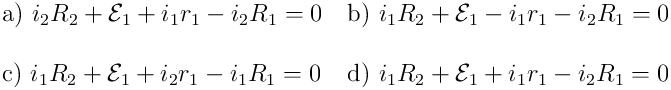
\includegraphics[width=2in]{picture.png}
\caption{ \label{fig:pic2} This is another example figure.}
\end{figure}

\vspace{1in}If you need more spacing,
  
just embed latex spacing commands.

\begin{minipage}{\linewidth}
  \begin{easylist}
  &  \label{prob_7} These questions are just to fill the page... 
    &&  \label{prob_7_1} to show how page breaks work... 
    &&  \label{prob_7_2} questions should not be split across pages... 
    &&  \label{prob_7_3} the main question and all parts should appear on the same page. 
    &&  \label{prob_7_4} so, yea. Figures \ref{fig:pic1} and \ref{fig:pic2} are the same. 
  \end{easylist}
\end{minipage}
\begin{minipage}{\linewidth}
  \begin{easylist}
  &  \label{prob_8} These questions are just to fill the page... 
    &&  \label{prob_8_1} to show how page breaks work... 
    &&  \label{prob_8_2} questions should not be split across pages... 
    &&  \label{prob_8_3} the main question and all parts should appear on the same page. 
    &&  \label{prob_8_4} so, yea. Figures \ref{fig:pic1} and \ref{fig:pic2} are the same. 
  \end{easylist}
\end{minipage}
\begin{minipage}{\linewidth}
  \begin{easylist}
  &  \label{prob_9} These questions are just to fill the page... 
    &&  \label{prob_9_1} to show how page breaks work... 
    &&  \label{prob_9_2} questions should not be split across pages... 
    &&  \label{prob_9_3} the main question and all parts should appear on the same page. 
    &&  \label{prob_9_4} so, yea. Figures \ref{fig:pic1} and \ref{fig:pic2} are the same. 
  \end{easylist}
\end{minipage}
\begin{minipage}{\linewidth}
  \begin{easylist}
  &  \label{prob_10} These questions are just to fill the page... 
    &&  \label{prob_10_1} to show how page breaks work... 
    &&  \label{prob_10_2} questions should not be split across pages... 
    &&  \label{prob_10_3} the main question and all parts should appear on the same page. 
    &&  \label{prob_10_4} so, yea. Figures \ref{fig:pic1} and \ref{fig:pic2} are the same. 
  \end{easylist}
\end{minipage}
\begin{minipage}{\linewidth}
  \begin{easylist}
  &  \label{prob_11} These questions are just to fill the page... 
    &&  \label{prob_11_1} to show how page breaks work... 
    &&  \label{prob_11_2} questions should not be split across pages... 
    &&  \label{prob_11_3} the main question and all parts should appear on the same page. 
    &&  \label{prob_11_4} so, yea. Figures \ref{fig:pic1} and \ref{fig:pic2} are the same. 
  \end{easylist}
\end{minipage}
\begin{minipage}{\linewidth}
  \begin{easylist}
  &  \label{prob_12} These questions are just to fill the page... 
    &&  \label{prob_12_1} to show how page breaks work... 
    &&  \label{prob_12_2} questions should not be split across pages... 
    &&  \label{prob_12_3} the main question and all parts should appear on the same page. 
    &&  \label{prob_12_4} so, yea. Figures \ref{fig:pic1} and \ref{fig:pic2} are the same. 
  \end{easylist}
\end{minipage}
\begin{minipage}{\linewidth}
  \begin{easylist}
  &  \label{prob_13} These questions are just to fill the page... 
    &&  \label{prob_13_1} to show how page breaks work... 
    &&  \label{prob_13_2} questions should not be split across pages... 
    &&  \label{prob_13_3} the main question and all parts should appear on the same page. 
    &&  \label{prob_13_4} so, yea. Figures \ref{fig:pic1} and \ref{fig:pic2} are the same. 
  \end{easylist}
\end{minipage}
\begin{minipage}{\linewidth}
  \begin{easylist}
  &  \label{prob_14} These questions are just to fill the page... 
    &&  \label{prob_14_1} to show how page breaks work... 
    &&  \label{prob_14_2} questions should not be split across pages... 
    &&  \label{prob_14_3} the main question and all parts should appear on the same page. 
    &&  \label{prob_14_4} so, yea. Figures \ref{fig:pic1} and \ref{fig:pic2} are the same. 
  \end{easylist}
\end{minipage}
\begin{minipage}{\linewidth}
  \begin{easylist}
  &  \label{prob_15} These questions are just to fill the page... 
    &&  \label{prob_15_1} to show how page breaks work... 
    &&  \label{prob_15_2} questions should not be split across pages... 
    &&  \label{prob_15_3} the main question and all parts should appear on the same page. 
    &&  \label{prob_15_4} so, yea. Figures \ref{fig:pic1} and \ref{fig:pic2} are the same. 
  \end{easylist}
\end{minipage}
\begin{minipage}{\linewidth}
  \begin{easylist}
  &  \label{prob_16} These questions are just to fill the page... 
    &&  \label{prob_16_1} to show how page breaks work... 
    &&  \label{prob_16_2} questions should not be split across pages... 
    &&  \label{prob_16_3} the main question and all parts should appear on the same page. 
    &&  \label{prob_16_4} so, yea. Figures \ref{fig:pic1} and \ref{fig:pic2} are the same. 
  \end{easylist}
\end{minipage}

\end{document}
